\documentclass[journal,12pt,twocolumn]{IEEEtran}

\usepackage{setspace}
\usepackage{gensymb}
\usepackage{xcolor}
\usepackage{caption}
\singlespacing
\usepackage[cmex10]{amsmath}
\usepackage{mathtools}
\usepackage{hyperref}
\usepackage{amsthm}
\usepackage{mathrsfs}
\usepackage{txfonts}
\usepackage{stfloats}
\usepackage{cite}
\usepackage{cases}
\usepackage{subfig}
\usepackage{longtable}
\usepackage{multirow}
\usepackage{enumitem}
\usepackage{mathtools}
\usepackage{listings}
\usepackage{tikz}
\let\vec\mathbf
\DeclareMathOperator*{\Res}{Res}
\renewcommand\thesection{\arabic{section}}
\renewcommand\thesubsection{\thesection.\arabic{subsection}}
\renewcommand\thesubsubsection{\thesubsection.\arabic{subsubsection}}

\renewcommand\thesectiondis{\arabic{section}}
\renewcommand\thesubsectiondis{\thesectiondis.\arabic{subsection}}
\renewcommand\thesubsubsectiondis{\thesubsectiondis.\arabic{subsubsection}}
\hyphenation{op-tical net-works semi-conduc-tor}

\lstset{
language=Python,
frame=single, 
breaklines=true,
columns=fullflexible
}

\begin{document}
%

\theoremstyle{definition}
\newtheorem{theorem}{Theorem}[section]
\newtheorem{problem}{Problem}
\newtheorem{proposition}{Proposition}[section]
\newtheorem{lemma}{Lemma}[section]
\newtheorem{corollary}[theorem]{Corollary}
\newtheorem{example}{Example}[section]
\newtheorem{definition}{Definition}[section]
\newcommand{\BEQA}{\begin{eqnarray}}
\newcommand{\EEQA}{\end{eqnarray}}
\newcommand{\define}{\stackrel{\triangle}{=}}
\newcommand{\myvec}[1]{\ensuremath{\begin{pmatrix}#1\end{pmatrix}}}
\newcommand{\mydet}[1]{\ensuremath{\begin{vmatrix}#1\end{vmatrix}}}

\bibliographystyle{IEEEtran}

\providecommand{\nCr}[2]{\,^{#1}C_{#2}} % nCr
\providecommand{\nPr}[2]{\,^{#1}P_{#2}} % nPr
\providecommand{\mbf}{\mathbf}
\providecommand{\pr}[1]{\ensuremath{\Pr\left(#1\right)}}
\providecommand{\qfunc}[1]{\ensuremath{Q\left(#1\right)}}
\providecommand{\sbrak}[1]{\ensuremath{{}\left[#1\right]}}
\providecommand{\lsbrak}[1]{\ensuremath{{}\left[#1\right.}}
\providecommand{\rsbrak}[1]{\ensuremath{{}\left.#1\right]}}
\providecommand{\brak}[1]{\ensuremath{\left(#1\right)}}
\providecommand{\lbrak}[1]{\ensuremath{\left(#1\right.}}
\providecommand{\rbrak}[1]{\ensuremath{\left.#1\right)}}
\providecommand{\cbrak}[1]{\ensuremath{\left\{#1\right\}}}
\providecommand{\lcbrak}[1]{\ensuremath{\left\{#1\right.}}
\providecommand{\rcbrak}[1]{\ensuremath{\left.#1\right\}}}
\theoremstyle{remark}
\newtheorem{rem}{Remark}
\newcommand{\sgn}{\mathop{\mathrm{sgn}}}
\providecommand{\abs}[1]{\left\vert#1\right\vert}
\providecommand{\res}[1]{\Res\displaylimits_{#1}} 
\providecommand{\norm}[1]{\lVert#1\rVert}
\providecommand{\mtx}[1]{\mathbf{#1}}
\providecommand{\mean}[1]{E\left[ #1 \right]}
\providecommand{\fourier}{\overset{\mathcal{F}}{ \rightleftharpoons}}
\providecommand{\ztrans}{\overset{\mathcal{Z}}{ \rightleftharpoons}}

\providecommand{\system}{\overset{\mathcal{H}}{ \longleftrightarrow}}
\newcommand{\solution}{\noindent \textbf{Solution: }}
\providecommand{\dec}[2]{\ensuremath{\overset{#1}{\underset{#2}{\gtrless}}}}
\numberwithin{equation}{section}
\makeatletter
\@addtoreset{figure}{problem}
\makeatother

\let\StandardTheFigure\thefigure
\renewcommand{\thefigure}{\theproblem}

\def\putbox#1#2#3{\makebox[0in][l]{\makebox[#1][l]{}\raisebox{\baselineskip}[0in][0in]{\raisebox{#2}[0in][0in]{#3}}}}
     \def\rightbox#1{\makebox[0in][r]{#1}}
     \def\centbox#1{\makebox[0in]{#1}}
     \def\topbox#1{\raisebox{-\baselineskip}[0in][0in]{#1}}
     \def\midbox#1{\raisebox{-0.5\baselineskip}[0in][0in]{#1}}

\vspace{3cm}

\title{ Circuits and Transforms }
\author{ Sumanth N R }
\maketitle
\tableofcontents

\renewcommand{\thefigure}{\theenumi}
\renewcommand{\thetable}{\theenumi}

\bigskip

\begin{abstract}
This manual provides a simple introduction to Transforms
\end{abstract}


\section{Definitions}

\begin{enumerate}[label=\arabic*.,ref=\thesection.\theenumi]
\numberwithin{equation}{section}
\numberwithin{figure}{section}

\item The unit step function is 
	\begin{align} u(t) = \begin{cases}
		1 & t > 0 \\
		\frac{1}{2} & t = 0 \\
		0 & t < 0
	\end{cases} \end{align}

\item The Laplace transform of $g(t)$ is defined as 
	\begin{align}
		G(s) = \int_{-\infty}^{\infty} g(t) e^{-st}\, dt
	\end{align}

\end{enumerate}



\section{Laplace Transform}

\begin{enumerate}[label=\arabic*.,ref=\thesection.\theenumi]
\numberwithin{equation}{section}

\item
	In the circuit, the switch S is connected to position P for a long time so that the charge on the capacitor becomes $q_1 \, \mu C$. Then S is switched to position Q.  After a long time, the charge on the capacitor is
	$q_2 \, \mu C$.
	\begin{figure}[!ht]
		\centering
		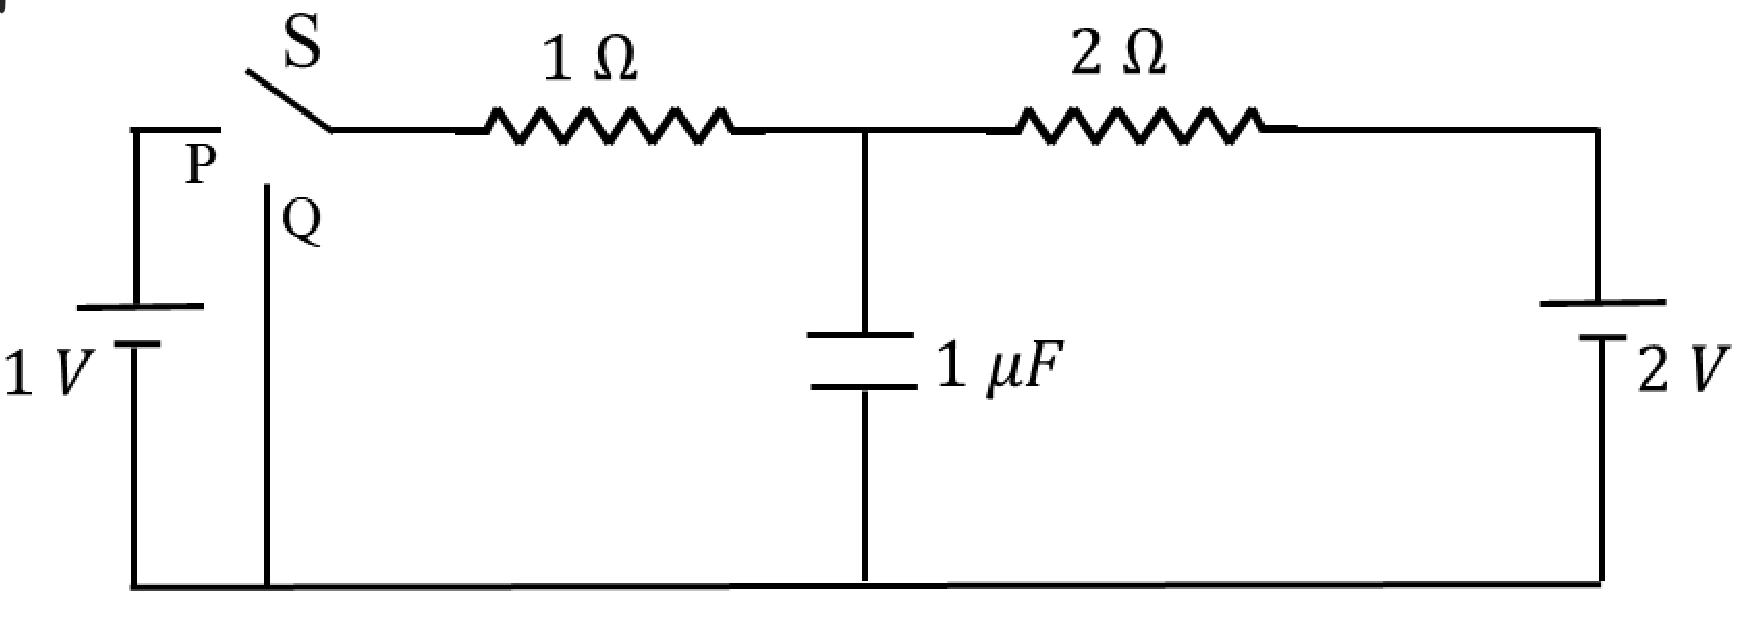
\includegraphics[width=\columnwidth]{../figs/ckt.jpg}
		\caption{}
		\label{fig:ckt}
	\end{figure}


\item Draw the circuit using latex-tikz.


\item Find $q_1$.


\item Show that the Laplace transform of $u(t)$ is $\frac{1}{s}$ and find the ROC.


\item Show that 
	\begin{align}
		e^{-at}u(t) \system{L} \frac{1}{s+a}, \quad a > 0
	\end{align}
	and find the ROC.


\item Now consider the following resistive circuit transformed from 
		Fig. \ref{fig:ckt}
	\begin{figure}[!ht]
		\centering
		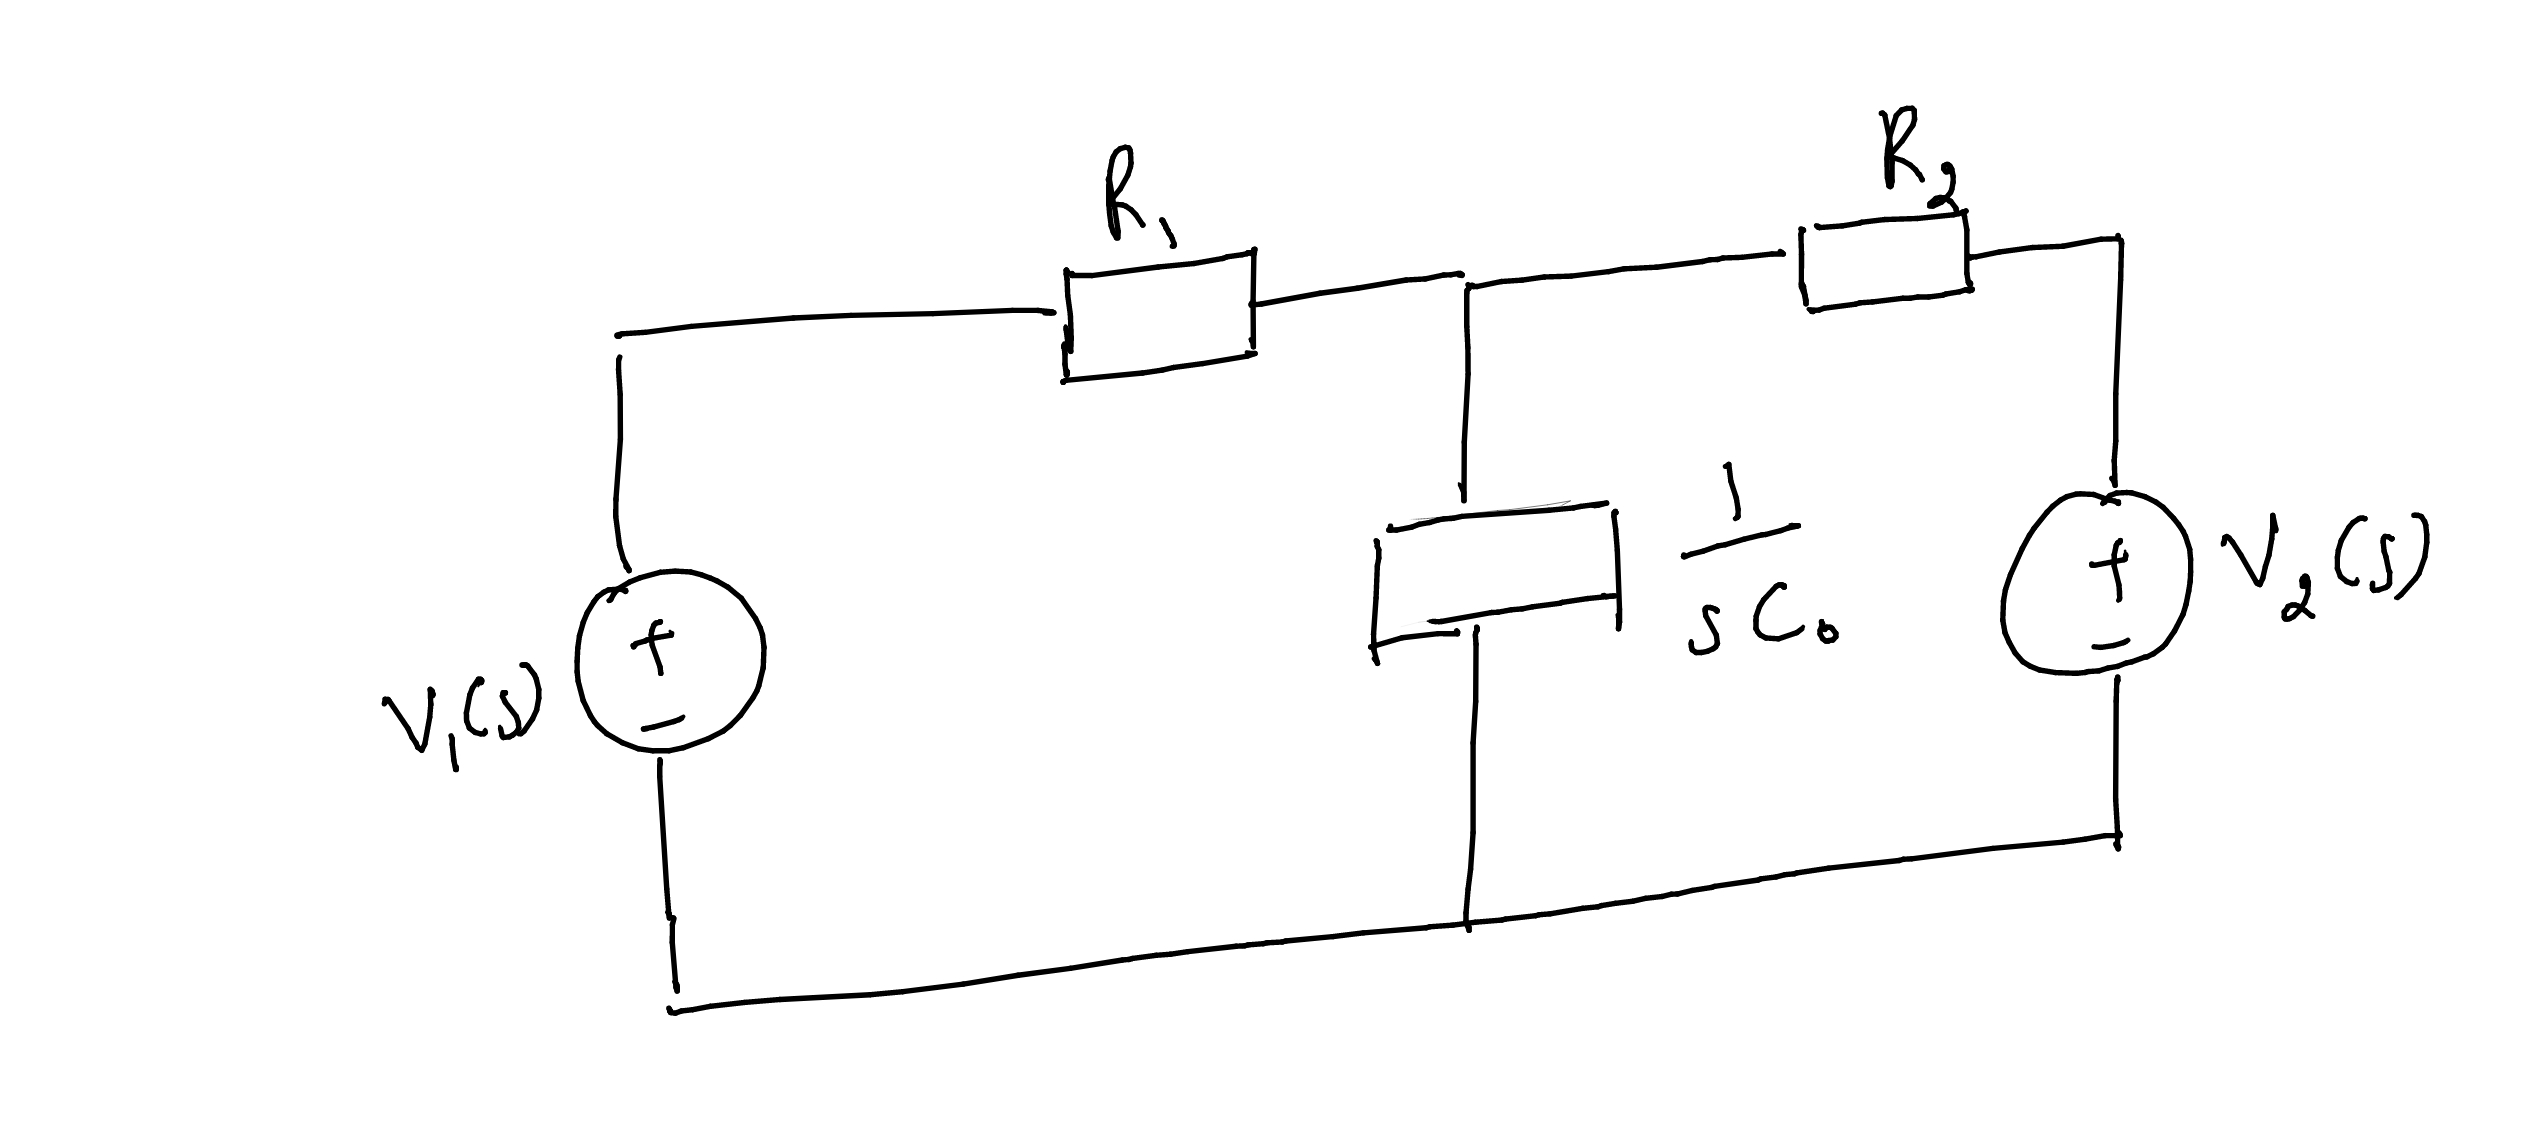
\includegraphics[width=\columnwidth]{../figs/lap-ckt.jpg}
		\caption{}
		\label{fig:lap-ckt}

	\end{figure}
		where 
		\begin{align}
			u(t) \system{L} V_1(s)
			\\
			2u(t) \system{L} V_2(s)
		\end{align}
		Find the voltage across the capacitor $V_{C_0}(s)$.
	
\item Find $v_{C_0}(t)$.  Plot using python.
\item Verify your result using ngspice.
\item Obtain Fig. 
			\ref{fig:lap-ckt}
			using the equivalent differential equation.
\end{enumerate}


\section{Initial Conditions}
\begin{enumerate}[label=\arabic*.,ref=\thesection.\theenumi]
\numberwithin{equation}{section}
\item Find $q_2$ in Fig. 
			\ref{fig:ckt}.
\item Draw the equivalent $s$-domain resistive circuit when S is switched to position Q.  Use variables $R_1, R_2, C_0$ for the passive elements.
Use latex-tikz.
		\label{prob:init}
	
		\item $V_{C_0}(s)$ = ?  
	\item $v_{C_0}(t)$ = ? Plot using python.
	\item Verify your result using ngspice.
	\item Find $v_{C_0}(0-), v_{C_0}(0+)$ and  $v_{C_0}(\infty) $. 
	\item Obtain the Fig.  in problem 
		\ref{prob:init}
			using the equivalent differential equation.


	\end{enumerate}

\end{document}
